


	\author{\textbf{Benjamin Andrea Schüpbach}\\ \\Matr.No. 14-100-564\\benjamin.schuepbach@students.unibe.ch\\Master's Student in Geography\\Institute of Geography, University of Bern\\}
	
	\date{\today}
	
	\title{\textbf{ICARUS\\}}
	\date{\today}
	
	
\thiswatermark{\centering \put(-1900,-1000){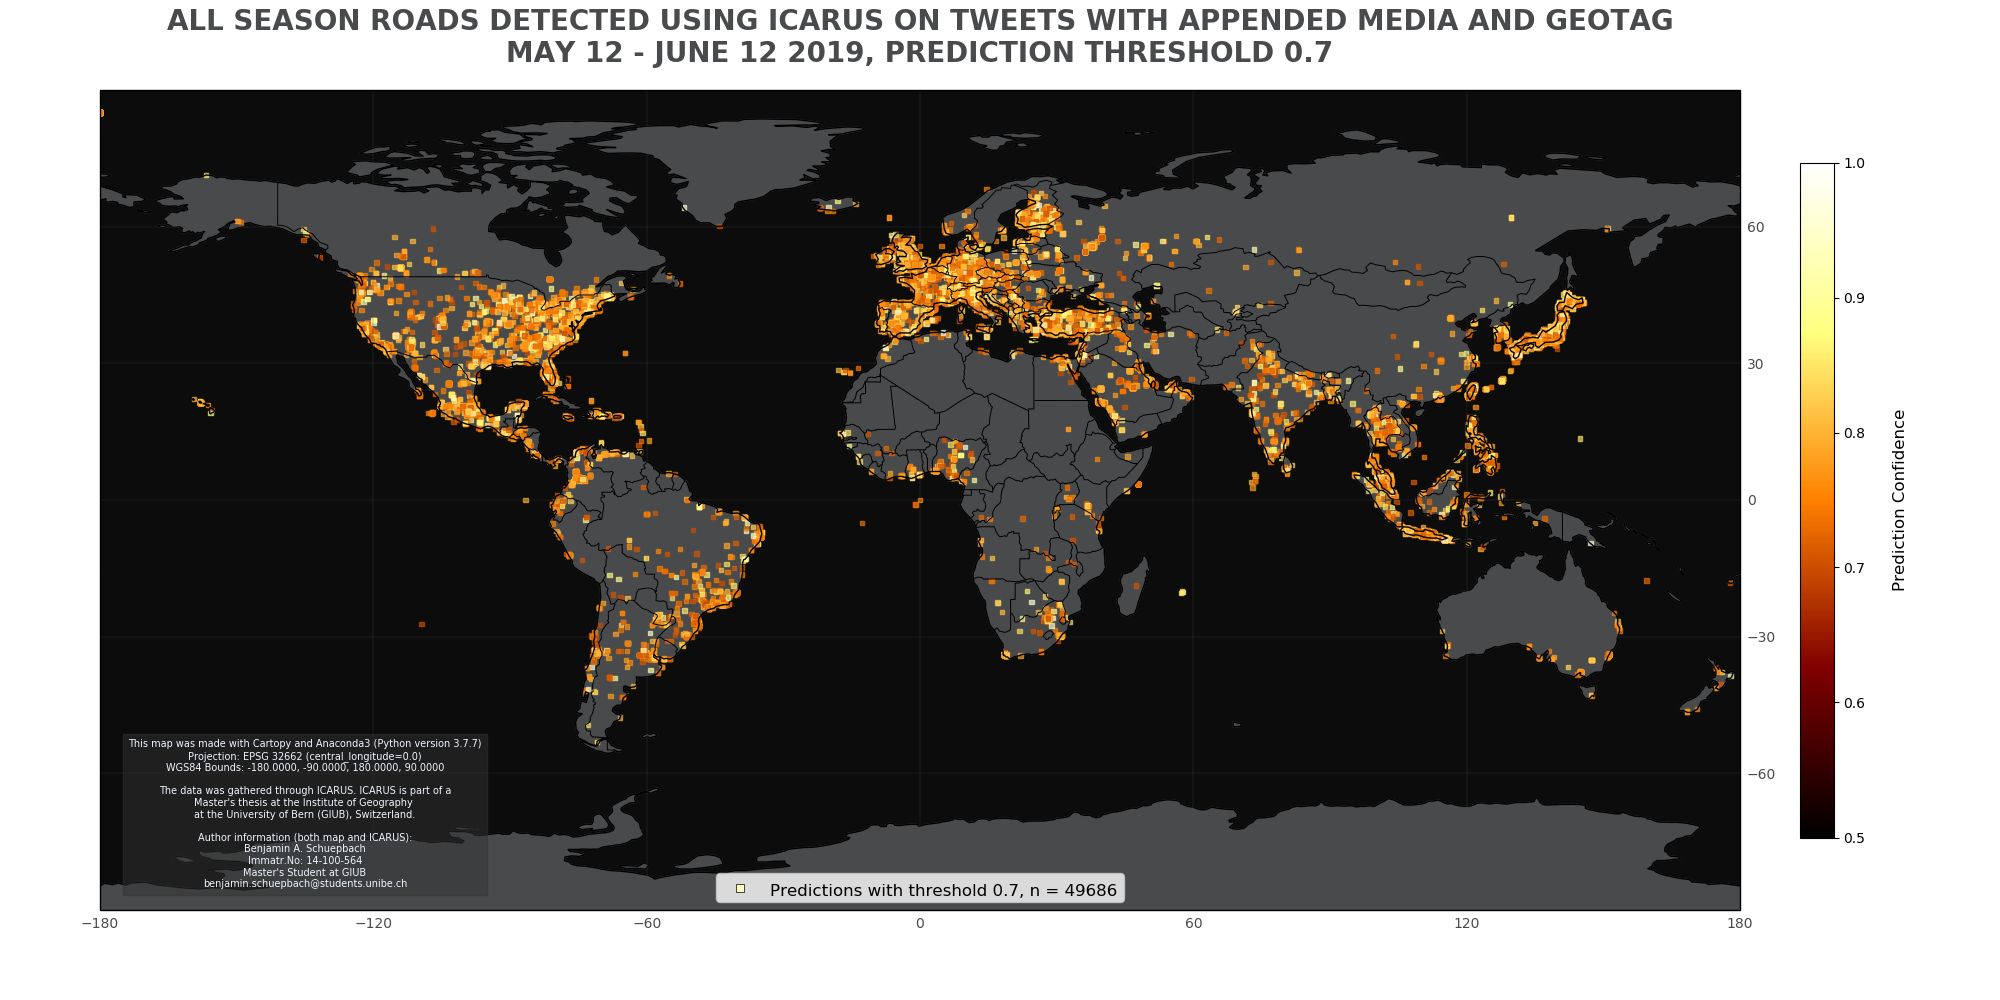
\includegraphics[scale=2]{images/map_ICARUS_thresh70.png}} }

\clearpage
\thispagestyle{empty}

\begin{tcolorbox}[standard jigsaw, opacityback=0.5, width=620, center]
	
	\begin{center}
	{\Huge \textbf{BIGGER IS BETTER. OR IS IT?}}\bigbreak
	\end{center}

	\begin{center}
		{\Large Lessons learned from using a Deep Neural Network to estimate Indicator \#58 of the Sustainable Development Goal's Agenda 2030.}
	\end{center}


\end{tcolorbox}



\begin{tcolorbox}[width=200, halign=left]
	Benjamin Andrea Schüpbach \bigbreak
	
	Matr.No. 14-100-564\smallbreak
	benjamin.schuepbach@students.unibe.ch\smallbreak
	Master's Student in Geography\smallbreak
	Institute of Geography, University of Bern
\end{tcolorbox}




\bigbreak
\bigbreak
\bigbreak
\bigbreak
\bigbreak
\bigbreak


\begin{center}
	Bern, XX.XX.2020
	\end{center}



\newpage